\documentclass[12pt]{article}
%%%%%%%%%%%%%%%%%%%%%%%%%%%%%%%%%%%%%%%%%%%%%%%%%%%%%%%%%%%%%%%%%%%%%%%%%%%%%%%%%%%%%
\usepackage[a4paper,margin=0.5in]{geometry}

\usepackage{titling}
\pretitle{\begin{center}\bfseries}
\posttitle{\end{center}}
\preauthor{\begin{center}}
\postauthor{\end{center}}
\predate{}
\postdate{}

\usepackage{titlesec}
\titleformat*{\section}{\bfseries}

\usepackage{caption}
\captionsetup{font=small,labelfont=bf}
\usepackage{floatrow}

\usepackage{graphicx}
\usepackage{epstopdf}
\epstopdfsetup{update,suffix=-generated}

\usepackage{hyperref}


%%%%%%%%%%%%%%%%%%%%%%%%%%%%%%%%%%%%%%%%%%%%%%%%%%%%%%%%%%%%%%%%%%%%%%%%%%%%%%%%%%%%%

\title{Optimal synaptic strategies for different timescales of memory}
\author{Subhaneil Lahiri and Surya Ganguli}
\date{}

%%%%%%%%%%%%%%%%%%%%%%%%%%%%%%%%%%%%%%%%%%%%%%%%%%%%%%%%%%%%%%%%%%%%%%%%%%%%%%%%%%%%%


\begin{document}

\pagestyle{empty}
\maketitle
\thispagestyle{empty}

%%%%%%%%%%%%%%%%%%%%%%%%%%%%%%%%%%%%%%%%%%%%%%%%%%%%%%%%%%%%%%%%%%%%%%%%%%%%%%%%%%%%%

Systems consolidation suggests that different brain regions are specialized to store memories over different timescales. Similarly, synapses mediating memory have highly complex, diverse molecular signaling pathways, varying across brain regions. This suggests the possibility that synaptic diversity across brain regions may be adapted for different timescales of memory storage. We are left with the fundamental question: what type of molecular synaptic dynamics is suitable for storing memory over any given timescale?

To address this, we systematically analyze an extremely broad class of models where synaptic plasticity is implemented by stochastic transitions between internal functional states of a sub-synaptic molecular network. Such models are essential in navigating stringent tradeoffs between learning and remembering, known as the stability-plasticity dilemma. Previous work (e.g.\ [Fusi, Drew, Abbott, 2005]) analyzed this tradeoff in models with only one topological structure of transitions between sub-synaptic states.  This leaves open the nature of this tradeoff over all possible sub-synaptic networks.  Rather than analyze one model, we analyze the space of all possible models and elucidate principles that determine how sub-synaptic network structure can be ideally adapted to the time-scale over which memories are stored.  We find that as this timescale increases, initially synapses are forced to grow a chain of internal states with rapid transitions, while at even longer timescales, synapses are further forced to exhibit slow stochastic transitions.

We also discuss the design of synaptic physiology experiments to test our theoretical predictions.  We find conventional methods for probing synaptic plasticity cannot discern the relevant synaptic dynamics.  Instead we propose new classes of experiments and data-analysis procedures in which more subtle protocols for probing plasticity can yield systems identification of the synaptic dynamics so crucial for storing memories at a particular time-scale.

%\section*{Additional Detail}
%
%We are extremely excited about this work as our theory allows us to relate two widely disparate observations: the systems consolidation of memories from one brain region to another and the diversity of sub-synaptic molecular networks across brain regions [Emes and Grant, 2012]. This provides us with a means to interpret, as well as predict, the nature of these differences in molecular architecture.
%
%We model the substructure of a synapse with a set of internal functional states that determine the synaptic weight, with plasticity inducing stochastic transitions between these states. We then look at the space of all possible transition topologies and transition probabilities. We combine rigorously proven theorems and numerical optimization to maximize a signal-to-noise ratio for memories as a function of the typical recall time for different brain regions. Finding the models that maximize this measure of memory at different timescales leads to an understanding of which structures are best suited for different memory timescales. The results can be seen in \autoref{fig:env}. We find that the optimal topology at each timescale has the states arranged in a chain. There are two qualitatively different mechanisms for preserving memory traces for longer times: (1) forcing the synapse to diffuse through a longer chain of states to change its strength and (2) lowering the transition rate between these states. We see that the first mechanism is used to go from short to intermediate timescales and the second mechanism is used to go from intermediate to long timescales.
%
%%\begin{SCfigure}
%%\caption{The memory curve envelope. This is an upper bound on the SNR as a function of the mean recall time for any model at each individual timescale. Thus no model, no matter what its transition topology between functional states, can have a memory curve that exceeds this envelope at any given time-scale. The models that achieve this upper bound are indicated at various timescales. The number of synapses is N and the number of internal functional states of each synapse is M. }\label{fig:env}
%%\includegraphics[width=0.6\linewidth]{LenvHeuristic.eps}
%%\end{SCfigure}
%\begin{figure}[t]
%\floatbox[{\capbeside\thisfloatsetup{capbesideposition={right,top},capbesidewidth=0.4\linewidth}}]{figure}{
%\caption{\textbf{The memory curve envelope.} This is an upper bound on the SNR as a function of the mean recall time for \textbf{\textit{any}} model at each individual timescale. Thus \textbf{\textit{no}} model, \emph{no matter what its transition topology between functional states}, can have a memory curve that exceeds this envelope at any given time-scale. The models that achieve this upper bound are indicated at various timescales. The number of synapses is $N$ and the number of internal functional states of each synapse is $M$. }\label{fig:env}}{
%\includegraphics[width=\linewidth]{LenvHeuristic.eps}}
%\end{figure}
%
%We believe that our approach of studying the entire space of models in this class is a vitally important one that should be much more widespread than it is. While studying individual models does have its own value, especially in revealing new ideas, it can be difficult to interpret without knowing how many other models can reproduce the same phenomena. Looking at all such models can uncover their essential features and lead to richer experimental predictions.
%
%The traditional style of synaptic plasticity experiments are designed to answer questions such as ``is this molecule/gene necessary/sufficient for LTP?'' Accordingly, the synapses are subjected to a protocol involving a large barrage of spikes that would ordinarily be guaranteed to induce plasticity. To test our predictions, instead one needs to take a Systems Identification approach, where the synapses are subjected to a long sequence of smaller stimuli that do not overwhelm the synapse’s internal dynamics. Then the correlations in the synaptic weight over longer timescales can be used to infer the structure of the latent states using Hidden Markov Model techniques, as seen in \autoref{fig:fit}. Overwhelming the system with large stimuli would hide these correlations, making it difficult to fit models. Given the radically different nature of these proposed experiments, we feel our work could have a substantial impact through interactions with, and feedback from, the Cosyne community.
%
%\begin{figure}[h]
%  \centering
%  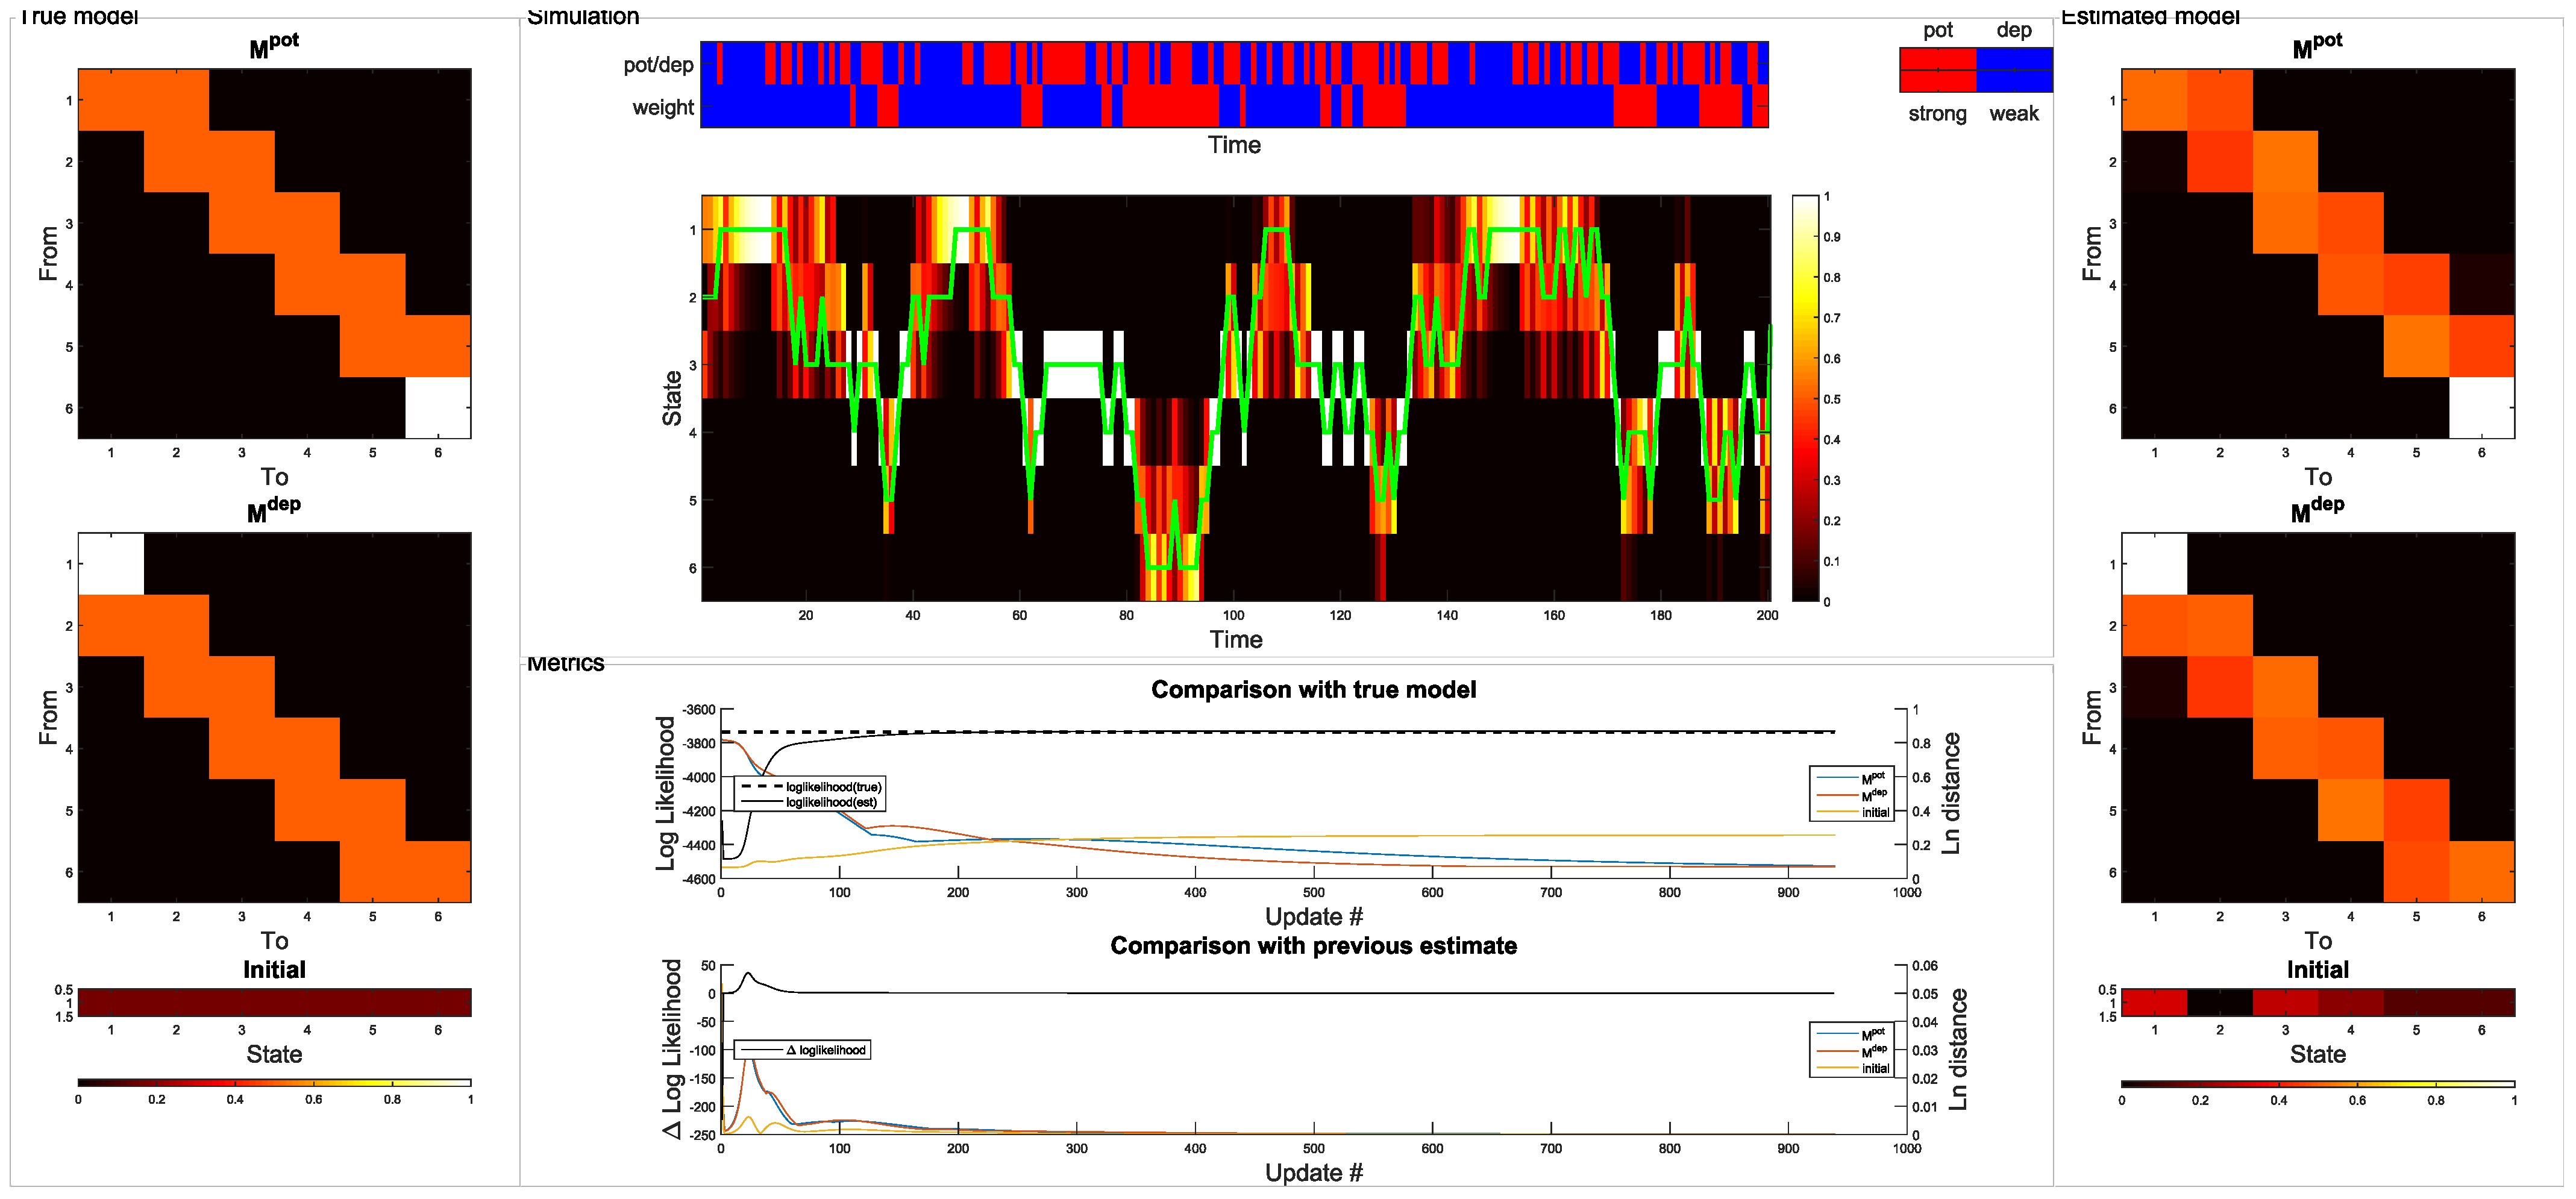
\includegraphics[width=0.99\linewidth]{FitVid939.eps}
%  \caption{\textbf{Simulated experiment for fitting synaptic models.} Left: the matrices of transition probabilities for the true model. Right: the result of the model fitting. Top middle: the sequence of potentiation/depotentiation the synapse is subjected to and the sequence of observed synaptic weights. Middle: the true sequence of synaptic states (green line) and the model’s estimated probability distribution (heat map).}\label{fig:fit}
%\end{figure}
%
%%%%%%%%%%%%%%%%%%%%%%%%%%%%%%%%%%%%%%%%%%%%%%%%%%%%%%%%%%%%%%%%%%%%%%%%%%%%%%%%%%%%%%
%
\end{document}




